\documentclass[12pt, a4paper]{article}
\usepackage[margin=1.25in]{geometry}
\usepackage{graphicx}
\usepackage{amsmath}
\usepackage{float}
\usepackage{listings}
\usepackage{physics}
\usepackage{mathrsfs}
\usepackage[shortlabels]{enumitem}


\setlength\parindent{0pt}
\newcommand{\code}{\lstinline[basicstyle=\small]}
\lstset{
    language=Python,
    basicstyle=\scriptsize
}


\title{EE2703: Applied Programming Lab \\ \Large Assignment 9: Spectra of Non-Periodic Signals}
\author{Soham Roy \\ \normalsize EE20B130}
\date{\today}
\begin{document}

\maketitle % Insert the title, author and date



\section{Introduction}
This assignment continues the examination of signals using Fourier Transforms, with non-periodic functions.
When these functions are periodically extended, discontinuities arise. Due to the Gibbs phenomenon, the discontinuities create
Fourier components in non-harmonic frequencies which decay as $\frac{1}{\omega}$. A Hamming window has been used to solve this
problem.



\section{Questions}
\subsection{Examples}
Spectrum of $\sin(\sqrt{2}t)$:
\begin{figure}[H]
    \centering
    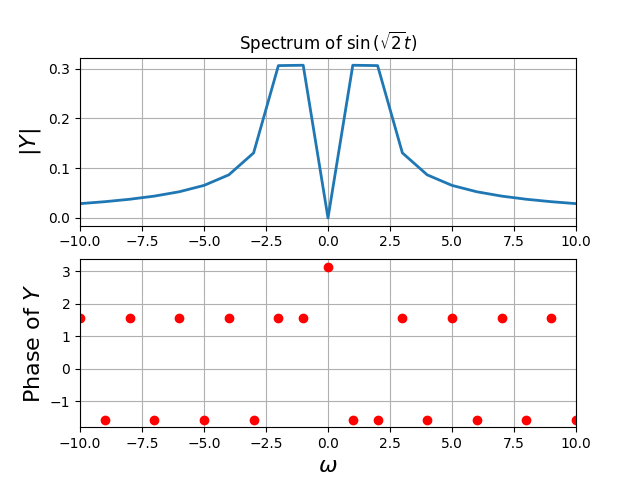
\includegraphics[scale=0.7]{eg1.png}
\end{figure}

Graph of $\sin(\sqrt{2}t)$:
\begin{figure}[H]
    \centering
    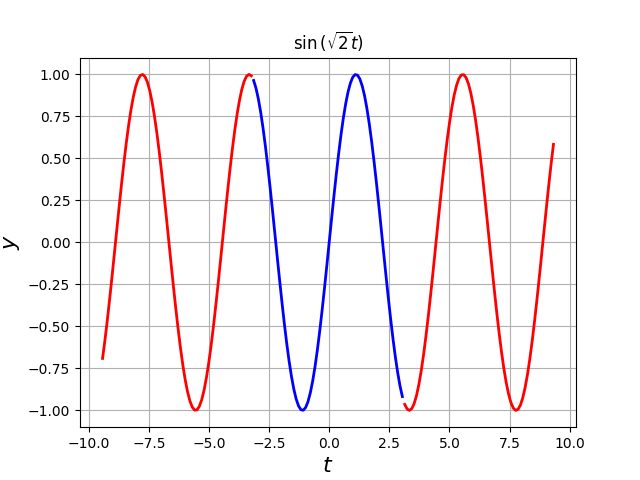
\includegraphics[scale=0.7]{eg2.png}
\end{figure}

$\sin(\sqrt{2}t)$ represented by the DFT:
\begin{figure}[H]
    \centering
    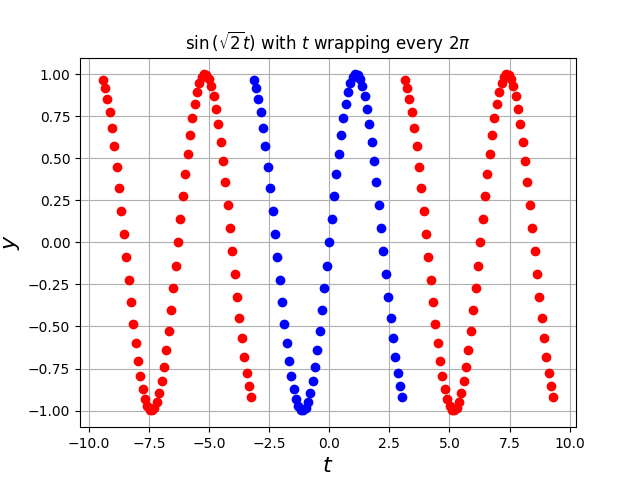
\includegraphics[scale=0.7]{eg3.png}
\end{figure}
\pagebreak

These discontinuities lead to non-harmonic components in the FFT which decay as $\frac{1}{\omega}$.
To confirm this, the spectrum of the periodic ramp has been plotted:
\begin{figure}[H]
    \centering
    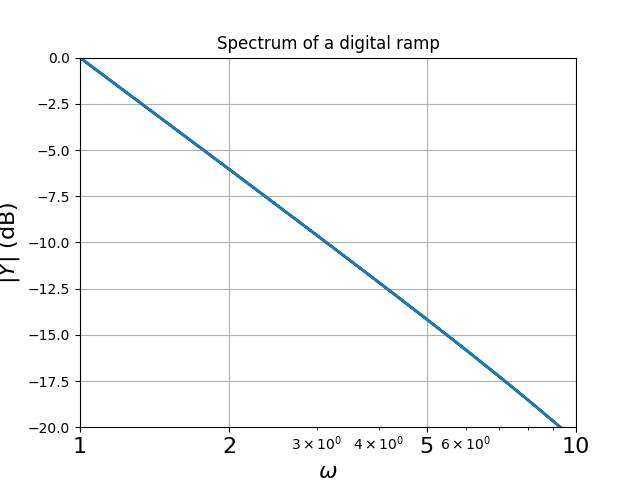
\includegraphics[scale=0.65]{eg4.png}
\end{figure}


\subsubsection{Hamming window}
The Hamming window removes discontinuities by attenuating the high frequency components that cause the discontinuities.
The Hamming window function is given by:
\begin{equation*}
    x[n] = 0.54 + 0.46\cos(\frac{2\pi n}{N - 1})
\end{equation*}

We now multiply our signal with the Hamming window and periodically extend it. We observe that the discontinuities nearly vanish:
\begin{figure}[H]
    \centering
    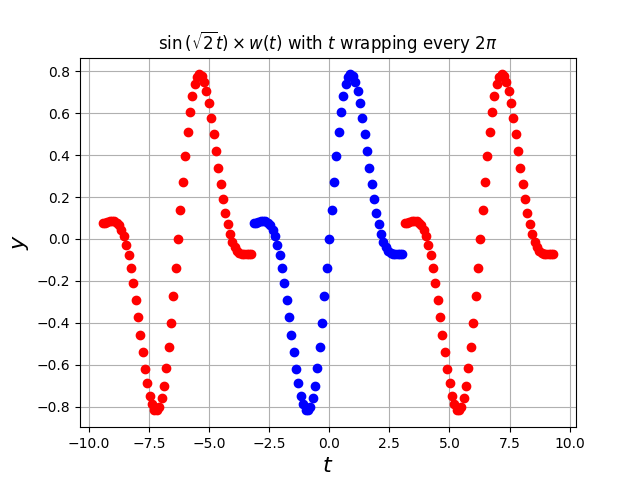
\includegraphics[scale=0.65]{eg5.png}
\end{figure}

The spectrum that is obtained with a time period $2\pi$ is given below:
\begin{figure}[H]
    \centering
    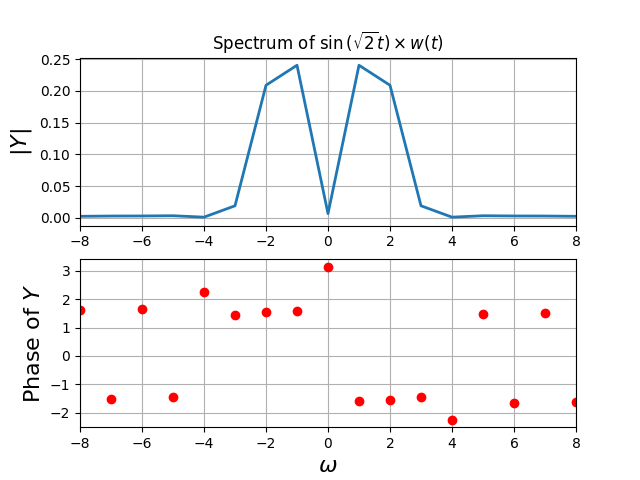
\includegraphics[scale=0.7]{eg6.png}
\end{figure}

The spectrum that is obtained with a time period $8\pi$ has a slightly sharper peak:
\begin{figure}[H]
    \centering
    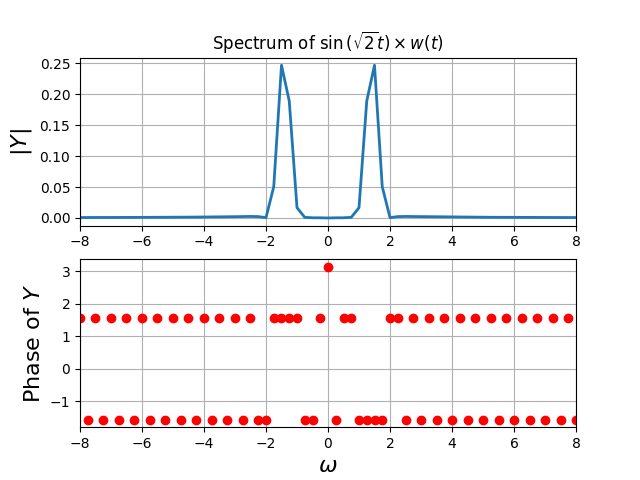
\includegraphics[scale=0.7]{eg7.png}
\end{figure}
\pagebreak


\section{Questions}
\subsection{Helper Functions}
We define the following helper functions:
\begin{lstlisting}
    def spectrum(f, n, lim, windowing=True, t=None):
        """Evaluates the DFT spectrum of a function f(t)."""
        if t is None:
            t, dt = np.linspace(-lim, lim, n, endpoint=False, retstep=True)
        else:
            dt = t[1] - t[0]
        f_max = 1 / dt
        w = np.linspace(-np.pi * f_max, np.pi * f_max, n, endpoint=False)
        y = f(t)
        if windowing:
            y *= fftshift(0.54 + 0.46 * np.cos(2 * np.pi * np.arange(n) / n))
        y[0] = 0  # the sample corresponding to -tmax should be set zero
        y = fftshift(y)  # make y start with y(t=0)
        Y = fftshift(fft(y)) / n

        return w, Y


    def plotter(w, Y, title, lim, out, xlabel, ylabels):
        """Plots the passed DFT spectrum."""
        plt.figure()
        plt.subplot(2, 1, 1)
        plt.title(title)
        plt.ylabel(ylabels[0], size=16)
        plt.plot(w, np.abs(Y), lw=2)
        plt.xlim(-lim, lim)
        plt.grid(True)

        plt.subplot(2, 1, 2)
        plt.xlabel(xlabel, size=16)
        plt.ylabel(ylabels[1], size=16)
        phase = np.angle(Y)
        phase[np.where(np.abs(Y) < 3e-3)] = 0
        plt.plot(w, phase, "ro", lw=2)
        plt.xlim(-lim, lim)
        plt.grid(True)

        plt.savefig("Assignment_09/LaTeX/" + out)
\end{lstlisting}


\subsection{Spectrum of $\cos^3(0.86t)$}
The FFT with and without the Hamming window have been plotted:
\begin{figure}[H]
    \centering
    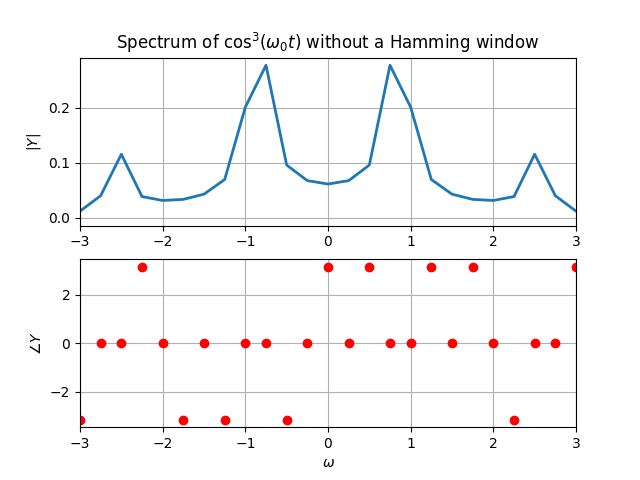
\includegraphics[scale=0.7]{q2a.png}
\end{figure}
\begin{figure}[H]
    \centering
    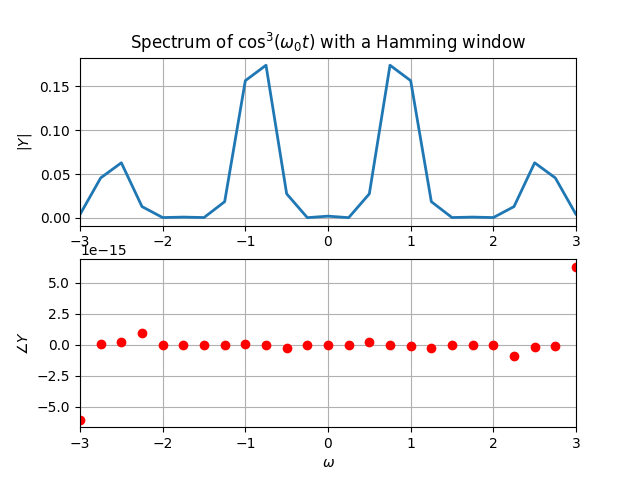
\includegraphics[scale=0.7]{q2b.png}
\end{figure}
It is observed that a large part of the energy is stored in frequencies that are not a part of the signal.
After windowing, these frequencies are attenuated and hence the peaks are sharper in the windowed function.
However, it is not an impulse because convolution with the Fourier transform of the windowed function smears out the peak.


\subsection{Estimate $\omega_0$ and $\delta$}\label{ssec:estimate}
We need to estimate $\omega_0$ and $\delta$ for a signal $\cos(\omega_0 t + \delta)$ for 128 samples between $[-\pi,\pi)$,
and find the two peaks at $\pm\omega_0$, and estimate $\omega_0$ and $\delta$. We estimate $\omega_0$ using a weighted average
over $|Y(\omega)|^2$, and $\delta$ is the phase at the frequency nearest to $\omega_0$.
\begin{lstlisting}
    def estimate_params(w, Y):
    """Estimates the parameters omega and delta of cos(omega*t + delta)."""
        ii = np.where(w > 0)
        omega = np.sum(np.abs(Y[ii]) ** 2 * w[ii]) / np.sum(np.abs(Y[ii]) ** 2)
        i = np.argmin(np.abs(w - omega))
        delta = np.angle(Y[i])
        
        return omega, delta
\end{lstlisting}
\begin{figure}[H]
    \centering
    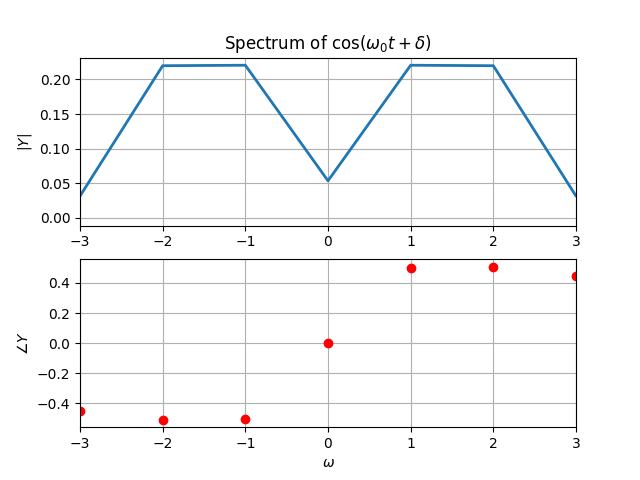
\includegraphics[scale=0.7]{q3.png}
\end{figure}


\subsection{$\cos^3(0.86t)$ with White Gaussian Noise}
We perform the same process as \ref{ssec:estimate} but with noise added to the original signal.
\begin{figure}[H]
    \centering
    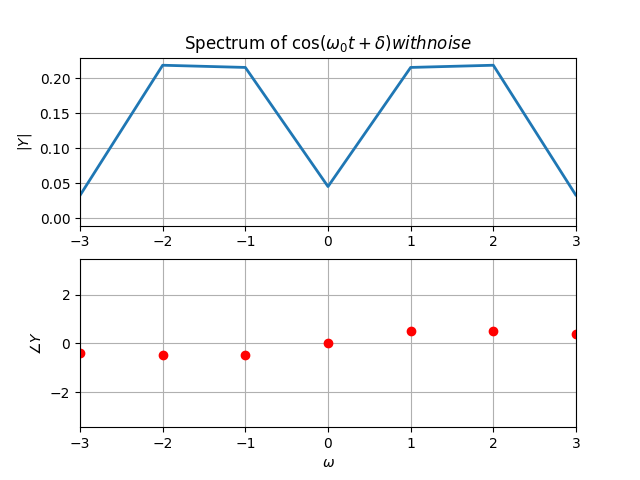
\includegraphics[scale=0.7]{q4.png}
\end{figure}

For the true value of $\omega_0 = 1.5$ and $\delta = 0.5$, the estimated values are:
\begin{lstlisting}
    Estimated w_0 = 1.516318, delta = 0.506776 without noise
    Estimated w_0 = 2.098451, delta = 0.481129 with noise
\end{lstlisting}


\subsection{DFT of Chirped Signal}
We analyze a chirp signal -- an FM signal where frequency is directly proportional to time:
\begin{equation*}
    f(t) = \cos(16t\left(1.5 + \frac{t}{2\pi}\right))
\end{equation*}

We observe that the frequency response is spread between 5 and 50 rad/s.
A large section of this range apears due to Gibbs phenomenon.
On windowing, only frequencies between 16 and 32 rad/s remain.
The FFT of the chirp is as follows:
\begin{figure}[H]
    \centering
    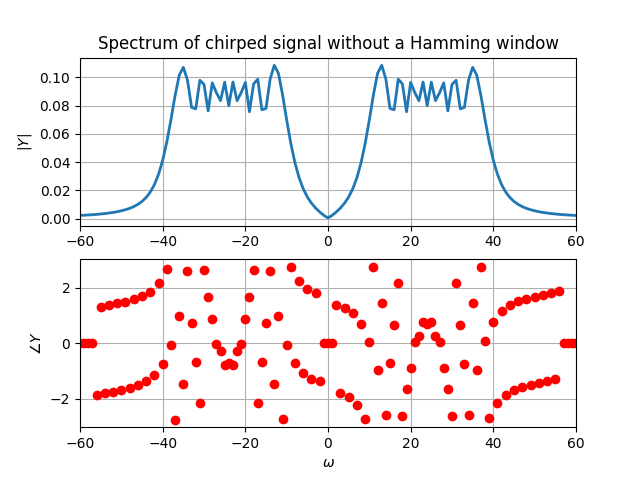
\includegraphics[scale=0.7]{q5a.png}
\end{figure}
\begin{figure}[H]
    \centering
    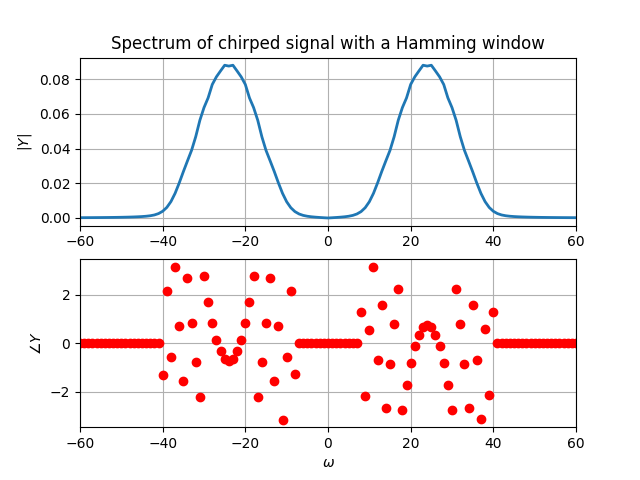
\includegraphics[scale=0.7]{q5b.png}
\end{figure}


\subsection{Surface Plot}
For the same chirped signal, the 1024 vector is broken into pieces that are 64 samples wide. Then we extract the
DFT of each and store as a column in a 2D array. Then we plot the array as a surface plot to show how the
frequency of the signal varies with time:
\begin{figure}[H]
    \centering
    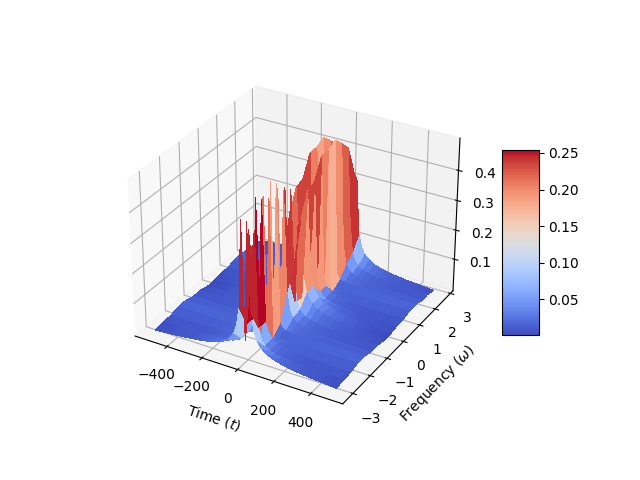
\includegraphics[scale=0.7]{q6.png}
\end{figure}


\section{Conclusion}
We investigated the need of windowing for DFTs in the case of non-periodic signals in this assignment.
This is done to reduce the effect of Gibbs phenomena caused by the discontinuous nature of the series
$\tilde{x}[n]$ generated by a discrete fourier transform.

The final question concerns chirped signals, in which we plot fourier spectra for various time slices of a
signal. We took more closely spaced slices after noticing the instance of a small number of slices.

The existence of two peaks, disappearing of chirp effects in case of a windowed transform, and a
phase plot that regularly varies with reduced phase near maximas are all visible aspects of a fourier spectra
for a chirped signal in time changing plots.



\end{document}
